% Provenance (never printed): cycle 4 SVT, "La planete Terre": sedimentation,
% from sediment to sedimentary rock, fossilisation, fossils and layers as a
% record of past environments; see sources/book1/PROVENANCE.md. Book 1,
% grade 7, chapter 4.
% Vocabulary guard: first chapter allowed to use "sediment"; the principles of
% relative dating (superposition, fossil succession and the rest) and "unconformity" are
% g7.5's and are not named here; fossils as evidence of evolution are the
% biology books' (one sentence of prose).
\chapter{Sédiments et fossiles}\label{ch:g7:sediments-and-fossils}

Le Grand Canyon, en Arizona (États-Unis), a une profondeur moyenne de
\qty{1.6}{km}. Ses parois sont faites de couches de \omterm{def:g3:stones-pebbles-sand:rock}{roche} posées les unes
sur les autres, rouges, brunes, grises et crème. Dans la couche du sommet,
le calcaire de Kaibab, les gardes du parc montrent des coquilles~: celles
de brachiopodes, des animaux qui vivaient sur le fond d'une \omterm{def:g2:water-on-earth:ocean}{mer}. Cette
\omterm{def:g3:stones-pebbles-sand:rock}{roche} s'est formée au fond d'un \omterm{def:g2:water-on-earth:ocean}{océan}, et elle forme aujourd'hui le bord
du canyon, bien au-dessus du \omterm{def:g4:world-physical-map:altitude}{niveau de la mer}.
% ledger: nps:grca-depth, nps:grca-fossils, nps:grca-kaibab

\begin{omfigure}
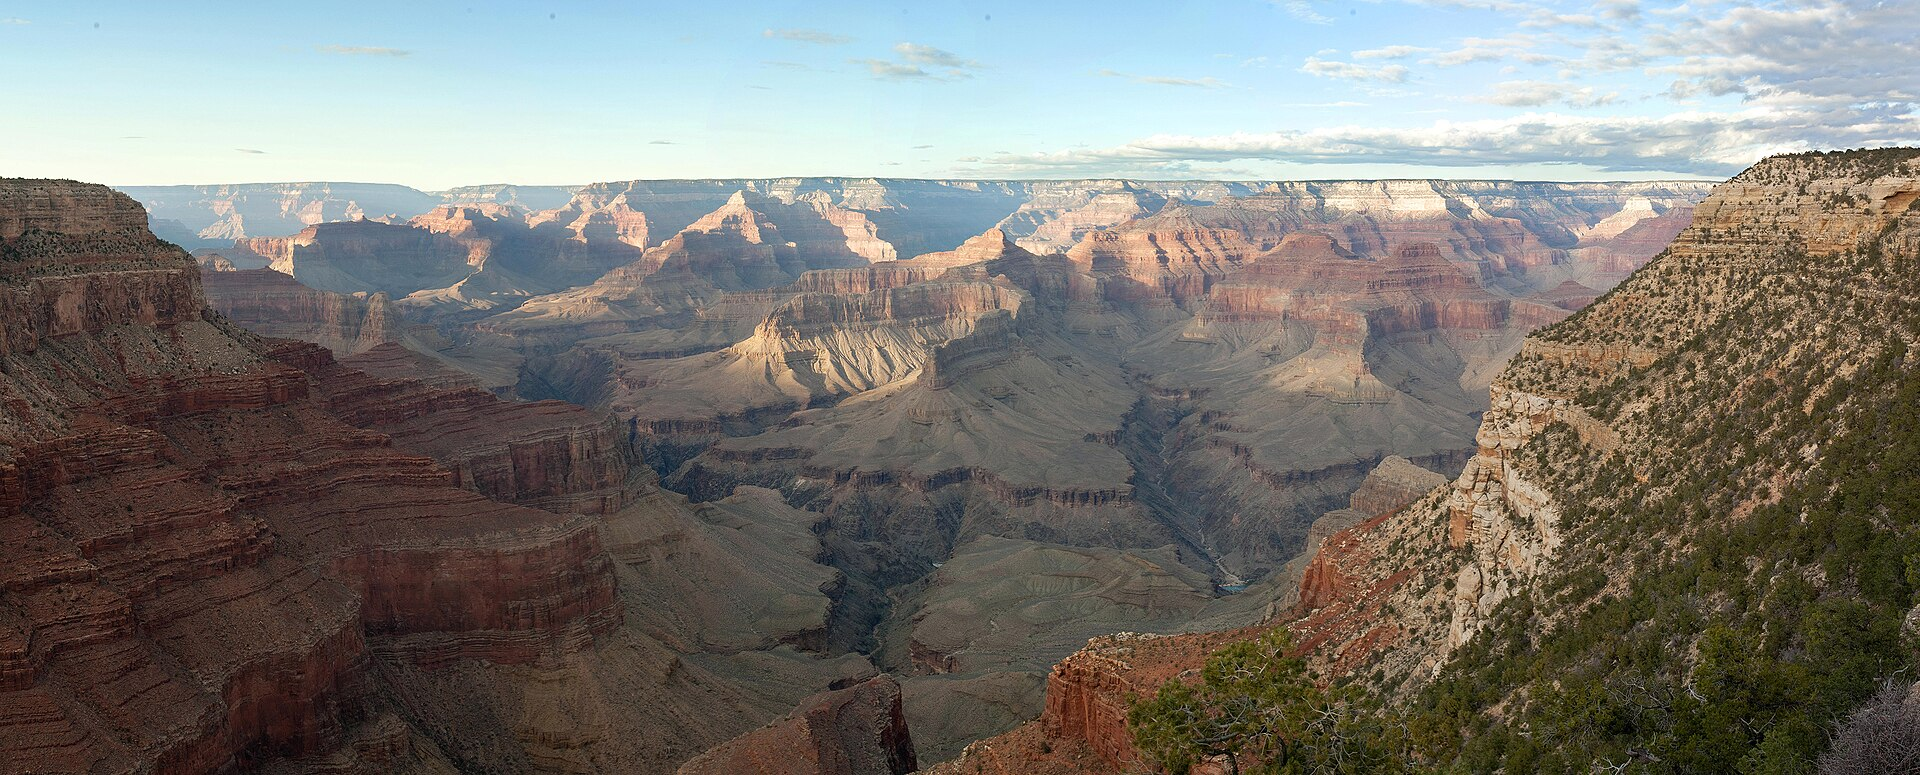
\includegraphics[width=\linewidth]{images/book1/g7-grand-canyon.jpg}

{\small Le Grand Canyon vu de Hermits Rest, sur son bord sud~: couche après
couche de \omterm{def:g3:stones-pebbles-sand:rock}{roche}, du bord jusqu'au fond. Photographie du NPS, par Kristen
M. Caldon (domaine public, via Wikimedia Commons).}
% ledger: commons:grand-canyon
\label{fig:g7:sediments-and-fossils:canyon}
\end{omfigure}

Comment un tas de \omterm{def:g3:stones-pebbles-sand:sand}{sable} et de \omterm{def:g3:stones-pebbles-sand:sand}{boue} meubles devient-il de la \omterm{def:g3:stones-pebbles-sand:rock}{roche}
solide~? Comment une coquille peut-elle durer si longtemps qu'elle finit
dans une falaise~? Et que nous disent les couches et les \omterm{def:g7:sediments-and-fossils:fossil}{fossiles} sur les
lieux tels qu'ils étaient il y a très longtemps~?

\begin{recall}
À la surface, les \omterm{def:g3:stones-pebbles-sand:rock}{roches} sont lentement brisées en morceaux
(\emph{\omterm{def:g5:water-shapes-the-land:weathering}{altération}})~; l'eau, le vent et la glace emportent les morceaux
(\emph{\omterm{def:g5:water-shapes-the-land:erosion}{érosion}}) et les déposent là où ils ralentissent et s'arrêtent
(\emph{\omterm{def:g5:water-shapes-the-land:deposition}{dépôt}})~: les plus lourds d'abord, la \omterm{def:g3:stones-pebbles-sand:sand}{boue} fine seulement là où
l'eau est presque immobile (\cref{ch:g5:water-shapes-the-land}). Une
\emph{\omterm{def:g6:rocks-and-minerals:rock-families}{roche sédimentaire}} se forme à la surface à partir de grains de
\omterm{def:g3:stones-pebbles-sand:sand}{sable} et de \omterm{def:g3:stones-pebbles-sand:sand}{boue}, ou de coquilles, déposés en couches puis durcis~: le
grès, l'argilite, le calcaire. Le \omterm{def:g6:rocks-and-minerals:rock-cycle}{cycle des roches} transforme lentement les
\omterm{def:g3:stones-pebbles-sand:rock}{roches} de chaque famille en \omterm{def:g3:stones-pebbles-sand:rock}{roches} des autres familles
(\cref{ch:g6:rocks-and-minerals}).
\end{recall}

\section{Les sédiments se déposent en couches}

Partout où l'eau, le vent ou la glace lâchent ce qu'ils transportaient, un
\omterm{def:g5:water-shapes-the-land:deposition}{dépôt} meuble s'accumule~: du gravier et du \omterm{def:g3:stones-pebbles-sand:sand}{sable} dans le lit d'une \omterm{def:g1:landscapes-around-us:water}{rivière},
de la \omterm{def:g3:stones-pebbles-sand:sand}{boue} au fond d'un \omterm{def:g1:landscapes-around-us:water}{lac}, du \omterm{def:g3:stones-pebbles-sand:sand}{sable} sur une plage ou dans une dune, des
coquilles sur le fond de la \omterm{def:g2:water-on-earth:ocean}{mer}.

\begin{definition}[Sédiment]\label{def:g7:sediments-and-fossils:sediment}
Un \emph{sédiment}\index{sediment@sédiment} est un matériau meuble déposé
par l'eau, le vent ou la glace~: du gravier, du \omterm{def:g3:stones-pebbles-sand:sand}{sable}, de la \omterm{def:g3:stones-pebbles-sand:sand}{boue}, ou les
coquilles et les squelettes d'êtres vivants. Il s'accumule au fond des
\omterm{def:g1:landscapes-around-us:water}{rivières}, des \omterm{def:g1:landscapes-around-us:water}{lacs} et des \omterm{def:g2:water-on-earth:ocean}{mers}, et sur la terre ferme, là où le vent ou la
glace le lâchent.
\end{definition}

Les \omterm{def:g7:sediments-and-fossils:sediment}{sédiments} se déposent dans un ordre précis. Quand une eau boueuse
ralentit, les grains les plus gros et les plus lourds tombent au fond les
premiers, et les plus petits et les plus légers en dernier. Chaque fois que
l'eau change --- une \omterm{def:g5:water-shapes-the-land:flood}{crue} qui apporte du \omterm{def:g3:stones-pebbles-sand:sand}{sable}, puis des semaines calmes
pendant lesquelles seule la \omterm{def:g3:stones-pebbles-sand:sand}{boue} fine atteint le fond ---, les grains qui
se déposent changent aussi, et une nouvelle couche commence. Peu à peu, le
fond d'un \omterm{def:g1:landscapes-around-us:water}{lac} ou d'une \omterm{def:g2:water-on-earth:ocean}{mer} se couvre d'une pile de couches, la plus
ancienne en bas de la pile.
% ledger: usgs:strata, usgs:sediments-to-rock

\begin{omfigure}
\begin{tikzpicture}[font=\small, x=1cm, y=1cm]
  % land and river
  \fill[omLithAlluv] (0,3.0) -- (2.0,2.45) -- (2.0,0) -- (0,0) -- cycle;
  \fill[blue!35] (0,3.05) -- (2.0,2.5) -- (2.0,2.4) -- (0,2.95) -- cycle;
  % lake water
  \fill[omSea!45] (2.0,2.5) -- (12.4,2.5) -- (12.4,1.12) -- (3.0,1.2) -- cycle;
  \draw[blue!50!black, line width=0.6pt] (2.0,2.5) -- (12.4,2.5);
  % layers on the bottom: thick near the mouth, thinner far out
  \foreach \k/\c in {0/omLithSand, 1/omLithShale, 2/omLithSand, 3/omLithShale} {
    \pgfmathsetmacro{\yb}{0.2+0.25*\k}
    \pgfmathsetmacro{\yt}{0.2+0.25*(\k+1)}
    \fill[\c] (3.0,\yb) -- (12.4,\yb) -- (12.4,\yt-0.08) -- (3.0,\yt) -- cycle;
  }
  \draw[black!60, line width=0.3pt] (3.0,1.2) -- (12.4,1.12);
  \fill[omLithAlluv!80!black] (2.0,0) rectangle (12.4,0.2);
  \fill[omLithAlluv] (2.0,0.2) -- (3.0,0.2) -- (3.0,1.2) -- (2.0,2.45) -- cycle;
  % settling grains: big ones near the mouth, fine ones far out
  \foreach \x/\y in {3.3/2.1, 3.6/1.75, 3.9/2.25, 4.2/1.55, 3.5/1.35, 4.5/2.0} {
    \fill[brown!70!black] (\x,\y) circle (0.07);
    \draw[-{Stealth[length=1.3mm]}, black!60] (\x,\y-0.1) -- (\x,\y-0.32);
  }
  \foreach \x/\y in {6.5/2.2, 7.4/1.8, 8.3/2.15, 9.1/1.6, 9.9/2.05, 10.8/1.75, 11.6/2.1, 7.9/1.35, 10.4/1.3} {
    \fill[brown!50!black] (\x,\y) circle (0.025);
    \draw[-{Stealth[length=1mm]}, black!40] (\x,\y-0.05) -- (\x,\y-0.2);
  }
  \node[anchor=south, align=center] at (1.0,3.1) {une rivière en crue\\[-2pt]apporte sable et boue};
  \node[anchor=south, align=center] at (4.1,2.55) {le sable se dépose\\[-2pt]d'abord, près de l'embouchure};
  \node[anchor=south, align=center] at (9.2,2.55) {la boue fine se dépose lentement,\\[-2pt]au large, là où l'eau est calme};
  \draw[decorate, decoration={brace, amplitude=4pt}] (12.55,1.15) -- (12.55,0.2)
    node[midway, anchor=west, xshift=4pt, align=left, font=\footnotesize] {couches du\\[-2pt]fond~: sable,\\[-2pt]boue, sable, boue};
\end{tikzpicture}

{\small Des \omterm{def:g7:sediments-and-fossils:sediment}{sédiments} qui se déposent dans un \omterm{def:g1:landscapes-around-us:water}{lac} (un dessin, pas à
l'échelle). Après chaque \omterm{def:g5:water-shapes-the-land:flood}{crue}, une couche de \omterm{def:g3:stones-pebbles-sand:sand}{sable} se dépose, puis de la
\omterm{def:g3:stones-pebbles-sand:sand}{boue} fine pendant les semaines calmes qui suivent~: couche après couche,
une pile se forme sur le fond.}
% ledger: usgs:strata
\label{fig:g7:sediments-and-fossils:lake}
\end{omfigure}

\begin{definition}[Couche sédimentaire]\label{def:g7:sediments-and-fossils:layer}
Une \emph{couche sédimentaire}\index{couche sedimentaire@couche sédimentaire},
ou \emph{strate}\index{strate} (du latin \emph{stratum}, «~chose étendue~»), est une nappe de \omterm{def:g7:sediments-and-fossils:sediment}{sédiment}, ou de la \omterm{def:g3:stones-pebbles-sand:rock}{roche}
qu'il est devenu, déposée en une seule fois. Elle a une base et un sommet,
et elle se distingue des couches situées au-dessus et au-dessous par la
taille de ses grains ou par ce dont elle est faite.
\end{definition}

Les \omterm{def:g7:sediments-and-fossils:sediment}{sédiments} se déposent à partir de l'eau ou de l'air~: ils se déposent
donc à plat, comme les pages d'un livre posé sur une table. Quand on trouve
des couches inclinées ou plissées, c'est que quelque chose les a déplacées
après leur formation. Les couches sont la marque la plus nette d'une \omterm{def:g6:rocks-and-minerals:rock-families}{roche
sédimentaire}~: tu les as vues dans les parois du Grand Canyon.
% ledger: usgs:strata, nps:grca-kaibab

\begin{inthelab}[Des couches dans un bocal (en classe, avec l'enseignant)]
Mets une poignée de gravier, deux poignées de \omterm{def:g3:stones-pebbles-sand:sand}{sable} et quelques cuillerées
de terre dans un grand bocal en verre~; remplis-le d'eau, ferme-le bien et
secoue-le. Pose-le et observe pendant quelques minutes~: le gravier atteint
le fond tout de suite, le \omterm{def:g3:stones-pebbles-sand:sand}{sable} un peu plus tard, et la \omterm{def:g3:stones-pebbles-sand:sand}{boue} fine garde
l'eau trouble pendant des heures. Le lendemain, ajoute encore un peu de
terre et de \omterm{def:g3:stones-pebbles-sand:sand}{sable}, secoue doucement, et laisse reposer. Combien de couches
comptes-tu~? Quels grains se trouvent au bas de chacune~?
\end{inthelab}

\section{Du sédiment à la roche}

Une couche ne reste pas longtemps au-dessus. D'autres couches se déposent
sur elle, puis d'autres encore, et elle est enfouie de plus en plus
profond. Sous le poids des couches qui la recouvrent, les grains sont
serrés les uns contre les autres et l'eau qui les sépare est chassée. L'eau
qui s'infiltre dans la pile laisse des \omterm{def:g6:rocks-and-minerals:mineral}{minéraux} entre les grains, un
ciment naturel qui les colle ensemble. Avec le temps, à mesure que d'autres
couches s'entassent et que de lentes transformations chimiques ont lieu, le
\omterm{def:g7:sediments-and-fossils:sediment}{sédiment} meuble du bas de la pile devient une \omterm{def:g3:stones-pebbles-sand:rock}{roche}.
% ledger: usgs:sediments-to-rock, usgs:sedimentary

Chaque sorte de \omterm{def:g7:sediments-and-fossils:sediment}{sédiment} donne sa propre \omterm{def:g3:stones-pebbles-sand:rock}{roche}.

\begin{center}
\small
\begin{tabular}{|l|l|}
\hline
\textbf{\omterm{def:g7:sediments-and-fossils:sediment}{sédiment}} & \textbf{la \omterm{def:g3:stones-pebbles-sand:rock}{roche} qu'il devient} \\
\hline
gravier et \omterm{def:g3:stones-pebbles-sand:pebble}{galets} & conglomérat \\
\omterm{def:g3:stones-pebbles-sand:sand}{sable} & grès \\
\omterm{def:g3:stones-pebbles-sand:sand}{boue} & pélite, ou argilite quand elle se débite en feuillets fins \\
coquilles et squelettes & calcaire \\
débris de plantes, enfouis dans un marécage & charbon \\
\hline
\end{tabular}
\end{center}
% ledger: usgs:sediments-to-rock, usgs:sedimentary, usgs:coal-origin

\begin{omfigure}
\begin{tikzpicture}[font=\small, x=1cm, y=1cm]
  \pgfmathsetseed{11}
  \foreach \p/\gap/\title in {0/0.40/{sédiment meuble}, 1/0.31/{enfoui et tassé~:\\[-2pt]l'eau est chassée}, 2/0.31/{cimenté~: une roche}} {
    \begin{scope}[xshift=\p*4.6cm]
      \ifnum\p=2 \fill[black!25] (0,0) rectangle (3.4,3.0);
      \else \fill[omSea!45] (0,0) rectangle (3.4,3.0); \fi
      \foreach \i in {0,...,7} {
        \foreach \j in {0,...,6} {
          \pgfmathsetmacro{\gx}{0.25 + \i*\gap*1.05 + 0.05*rand}
          \pgfmathsetmacro{\gy}{0.25 + \j*\gap + 0.05*rand}
          \pgfmathsetmacro{\gr}{0.13 + 0.03*rand}
          \ifdim\gx pt<3.25pt \ifdim\gy pt<2.85pt
            \fill[omLithSand!80!brown, draw=brown!60!black, line width=0.3pt] (\gx,\gy) circle (\gr);
          \fi\fi
        }
      }
      \draw[black!70, line width=0.6pt] (0,0) rectangle (3.4,3.0);
      \node[anchor=north, align=center] at (1.7,-0.1) {\title};
    \end{scope}
  }
  \draw[-{Stealth[length=2.5mm]}, line width=1pt] (3.6,1.5) -- (4.4,1.5);
  \draw[-{Stealth[length=2.5mm]}, line width=1pt] (8.2,1.5) -- (9.0,1.5);
  \foreach \x in {5.3,6.3,7.3} \draw[-{Stealth[length=2mm]}, line width=0.8pt] (\x,3.7) -- (\x,3.1);
  \node[anchor=south] at (6.3,3.7) {poids des couches du dessus};
  \node[anchor=south, font=\footnotesize, align=center] at (10.9,3.05) {en gris~: le ciment naturel};
\end{tikzpicture}

{\small Du \omterm{def:g3:stones-pebbles-sand:sand}{sable} au grès (un dessin des grains, très agrandis). À
gauche~: des grains meubles, avec de l'eau entre eux. Au milieu~: enfouis
sous de nouvelles couches, les grains sont serrés les uns contre les
autres. À droite~: des \omterm{def:g6:rocks-and-minerals:mineral}{minéraux} laissés par l'eau collent les grains
ensemble.}
% ledger: usgs:sediments-to-rock, usgs:sedimentary
\label{fig:g7:sediments-and-fossils:to-rock}
\end{omfigure}

La plupart des \omterm{def:g3:stones-pebbles-sand:rock}{roches} que l'on peut voir à la surface de la Terre sont
sédimentaires. La pile de couches qu'elles forment est le livre d'histoire
du lieu~: chaque couche est une page, et les pages les plus anciennes sont
en bas.
% ledger: usgs:sediments-to-rock

\section{Comment se forme un fossile}

\begin{definition}[Fossile]\label{def:g7:sediments-and-fossils:fossil}
Un \emph{fossile}\index{fossile} est le reste, ou la trace, d'un être vivant
d'autrefois, conservé dans la \omterm{def:g3:stones-pebbles-sand:rock}{roche}. Certains fossiles sont les parties
dures du corps --- une coquille, un os, une dent, du bois --- changées en
pierre. D'autres ne gardent qu'une forme~: un \emph{moule}\index{moule} est
l'empreinte en creux laissée dans la \omterm{def:g3:stones-pebbles-sand:rock}{roche} là où une coquille ou un os
s'est dissous~; un \emph{moulage}\index{moulage} est la copie qui se forme
quand un moule se remplit de nouvelle matière minérale ou de \omterm{def:g7:sediments-and-fossils:sediment}{sédiment}. Une
\emph{trace fossile}\index{trace fossile} est un signe de ce qu'un animal a
fait --- une empreinte de pas, un terrier, une piste --- et non une partie
de son corps.
\end{definition}

Un \omterm{def:g7:sediments-and-fossils:fossil}{fossile} commence sa vie comme un animal ou une plante mort, sur le fond
d'une \omterm{def:g2:water-on-earth:ocean}{mer} ou d'un \omterm{def:g1:landscapes-around-us:water}{lac}. S'il reste à découvert, les bactéries le
décomposent et l'eau dissout lentement ce qui reste. Il n'a une chance que
s'il est enfoui rapidement, sous un \omterm{def:g7:sediments-and-fossils:sediment}{sédiment} qui se dépose sur lui et
l'isole. Ensuite, pendant que le \omterm{def:g7:sediments-and-fossils:sediment}{sédiment} se change en \omterm{def:g3:stones-pebbles-sand:rock}{roche}, l'eau qui
s'infiltre dans les couches apporte des \omterm{def:g6:rocks-and-minerals:mineral}{minéraux} qui remplissent le
moindre petit trou de la coquille ou de l'os~: il se change en pierre.
Bien plus tard, les couches du dessus peuvent être usées, et le \omterm{def:g7:sediments-and-fossils:fossil}{fossile}
apparaît à la surface.
% ledger: ucmp:fossil-conditions, ucmp:fossil-kinds, usgs:sediments-to-rock

\begin{omfigure}
\begin{tikzpicture}[font=\small, x=0.86cm, y=0.86cm,
    shell/.pic={
      \fill[#1] (0,0) circle (0.42);
      \draw[brown!40!black, line width=0.5pt] plot[domain=0:12.5, samples=90, smooth]
        ({0.032*\x*cos(\x r)}, {0.032*\x*sin(\x r)});
      \draw[brown!40!black, line width=0.5pt] (0,0) circle (0.42);
    }]
  % 1: death on the sea floor
  \begin{scope}[xshift=0cm]
    \fill[omSea!45] (0,1.2) rectangle (3.3,3.6);
    \fill[omLithShale] (0,0) rectangle (3.3,1.2);
    \pic at (1.65,1.62) {shell=omLithSand!60!white};
    \node[anchor=north, align=center] at (1.65,-0.1) {1. il meurt sur\\[-2pt]le fond de la mer};
  \end{scope}
  % 2: quick burial
  \begin{scope}[xshift=3.75cm]
    \fill[omSea!45] (0,2.1) rectangle (3.3,3.6);
    \fill[omLithShale] (0,0) rectangle (3.3,1.2);
    \fill[omLithShale!70!white] (0,1.2) rectangle (3.3,2.1);
    \pic at (1.65,1.62) {shell=omLithSand!60!white};
    \foreach \x in {0.5,1.2,2.1,2.8} \fill[brown!50!black] (\x,2.4) circle (0.03);
    \node[anchor=north, align=center] at (1.65,-0.1) {2. la boue le\\[-2pt]recouvre vite};
  \end{scope}
  % 3: buried deep, turned to stone
  \begin{scope}[xshift=7.5cm]
    \fill[omLithShale!80!black] (0,0) rectangle (3.3,1.2);
    \fill[omLithShale!85!black] (0,1.2) rectangle (3.3,2.1);
    \fill[omLithSand] (0,2.1) rectangle (3.3,2.9);
    \fill[omLithLime] (0,2.9) rectangle (3.3,3.6);
    \pic at (1.65,1.62) {shell=black!35};
    \node[anchor=north, align=center] at (1.65,-0.1) {3. enfoui profond, il\\[-2pt]se change en pierre};
  \end{scope}
  % 4: uncovered by erosion
  \begin{scope}[xshift=11.25cm]
    \fill[white] (0,0) rectangle (3.3,3.6);
    \fill[omLithShale!80!black] (0,0) -- (3.3,0) -- (3.3,2.6) -- (2.4,2.3) -- (1.8,1.95) -- (1.2,1.7) -- (0,1.5) -- cycle;
    \draw[black!35, line width=0.4pt] (0,1.2) -- (3.3,1.2);
    \draw[black!60, line width=0.4pt] (0,1.5) -- (1.2,1.7) -- (1.8,1.95) -- (2.4,2.3) -- (3.3,2.6);
    \pic at (1.65,1.84) {shell=black!35};
    \node[anchor=north, align=center] at (1.65,-0.1) {4. l'érosion le\\[-2pt]ramène à la surface};
  \end{scope}
  \foreach \p in {0,1,2,3} {
    \begin{scope}[xshift=\p*3.75cm]
      \draw[black!70, line width=0.5pt] (0,0) rectangle (3.3,3.6);
    \end{scope}
  }
\end{tikzpicture}

{\small Comment se forme un \omterm{def:g7:sediments-and-fossils:fossil}{fossile} (un dessin, pas à l'échelle)~: une
coquille est vite enfouie sous la \omterm{def:g3:stones-pebbles-sand:sand}{boue}~; enfouie plus profond sous de
nouvelles couches, elle se change en pierre~; bien plus tard, l'\omterm{def:g5:water-shapes-the-land:erosion}{érosion} use
les couches du dessus et le \omterm{def:g7:sediments-and-fossils:fossil}{fossile} apparaît à la surface.}
% ledger: ucmp:fossil-conditions, ucmp:fossil-kinds
\label{fig:g7:sediments-and-fossils:steps}
\end{omfigure}

La plupart des êtres vivants ne laissent aucun \omterm{def:g7:sediments-and-fossils:fossil}{fossile}. Les corps mous
pourrissent avant d'avoir pu être enfouis~; même les coquilles et les os
se brisent ou se dissolvent s'ils restent longtemps à découvert. Le
meilleur endroit pour devenir un \omterm{def:g7:sediments-and-fossils:fossil}{fossile} est le fond d'une \omterm{def:g2:water-on-earth:ocean}{mer} ou d'un \omterm{def:g1:landscapes-around-us:water}{lac}
calme, où de la \omterm{def:g3:stones-pebbles-sand:sand}{boue} fine se dépose sur les restes et les protège. C'est
pourquoi les \omterm{def:g7:sediments-and-fossils:fossil}{fossiles} trouvés dans les \omterm{def:g3:stones-pebbles-sand:rock}{roches} sont surtout des coquilles,
ainsi que les minuscules coquilles et restes de plantes et d'animaux
microscopiques~; les dinosaures, les \omterm{def:g7:sediments-and-fossils:fossil}{fossiles} les plus célèbres, n'en sont
qu'une toute petite partie.
% ledger: ucmp:fossil-conditions, usgs:fossil-record-shells

\begin{omfigure}
\begin{minipage}[t]{0.49\linewidth}\centering
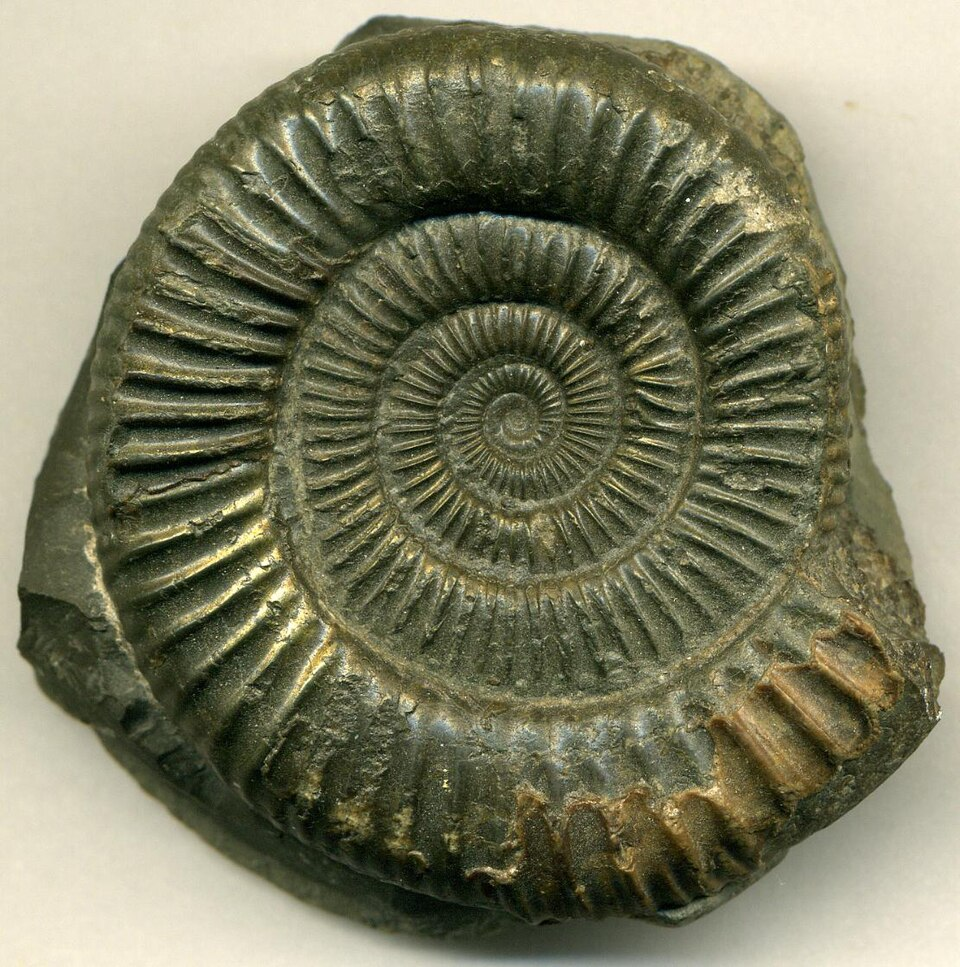
\includegraphics[height=4.6cm]{images/book1/g7-ammonite.jpg}

{\small Une ammonite, un animal disparu à coquille enroulée, parent des
calmars et des pieuvres, de \qty{5.7}{cm} de diamètre, de la \omterm{def:g1:landscapes-around-us:water}{côte} du
Yorkshire (Angleterre).}
\end{minipage}\hfill
\begin{minipage}[t]{0.49\linewidth}\centering
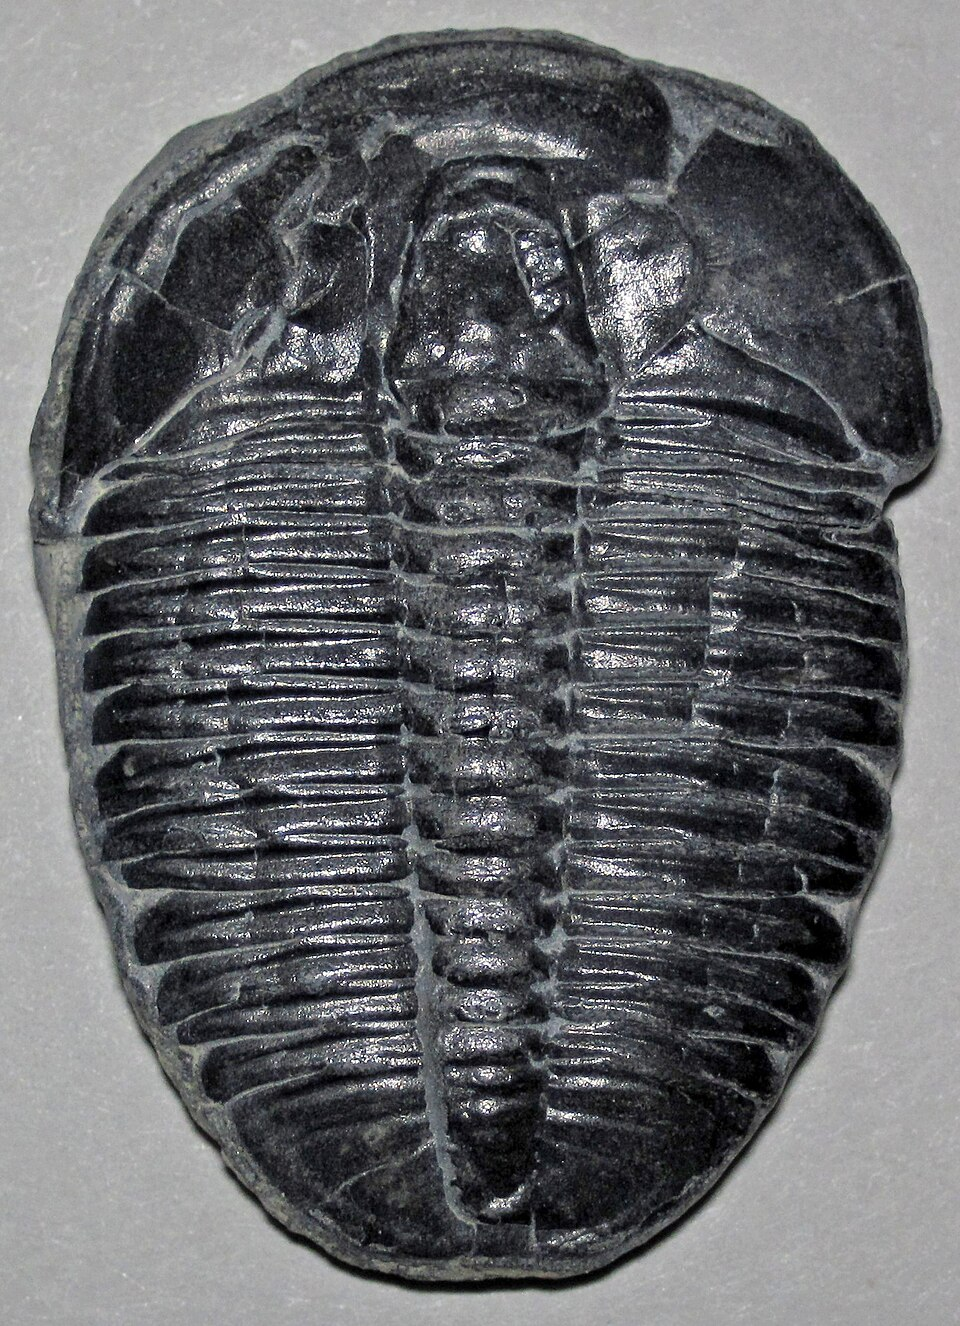
\includegraphics[height=4.6cm]{images/book1/g7-trilobite.jpg}

{\small Un trilobite, un animal marin disparu dont le corps a trois lobes,
d'environ \qty{2.6}{cm} de large, de l'Utah (États-Unis).}
\end{minipage}\par\medskip

{\small Deux \omterm{def:g7:sediments-and-fossils:fossil}{fossiles} d'animaux à coquille dure. Photographies~:
James St.~John (CC BY 2.0, via Wikimedia Commons).}
% ledger: commons:ammonite, commons:trilobite, nps:ammonoid, nps:trilobite
\label{fig:g7:sediments-and-fossils:ammonite-trilobite}
\end{omfigure}

Parfois, la coquille elle-même ne dure pas. Enfouie dans le \omterm{def:g3:stones-pebbles-sand:sand}{sable}, elle
est lentement dissoute par l'eau qui s'infiltre entre les grains, et il ne
reste qu'un creux, dont les parois portent la forme de la coquille~: un
\omterm{def:g7:sediments-and-fossils:fossil}{moule}. Si des \omterm{def:g6:rocks-and-minerals:mineral}{minéraux} se déposent plus tard dans le creux et le
remplissent, ils forment une copie de la coquille~: un \omterm{def:g7:sediments-and-fossils:fossil}{moulage}.
% ledger: ucmp:casts-molds

\begin{omfigure}
\begin{tikzpicture}[font=\small, x=1cm, y=1cm,
    clam/.style={line width=0.5pt}]
  \foreach \p/\fillc/\title in {0/{omLithSand!50!white}/{une coquille enfouie\\[-2pt]dans le sable}, 1/{white}/{la coquille s'est dissoute~:\\[-2pt]un moule}, 2/{black!40}/{des minéraux remplissent\\[-2pt]le moule~: un moulage}} {
    \begin{scope}[xshift=\p*4.9cm]
      \fill[omLithSand] (0,0) rectangle (4.2,2.6);
      \foreach \i in {0,...,40} {
        \pgfmathsetmacro{\gx}{0.1+mod(\i*0.53,4.0)}
        \pgfmathsetmacro{\gy}{0.1+mod(\i*0.37,2.4)}
        \fill[brown!60!black] (\gx,\gy) circle (0.025);
      }
      \fill[\fillc, draw=brown!40!black, clam] (0.9,0.9) arc[start angle=180, end angle=0, x radius=1.2, y radius=0.95] -- cycle;
      \ifnum\p=1
        \foreach \a in {25,45,...,155} \draw[brown!50!black, line width=0.4pt] (2.1,0.9) -- ++(\a:0.93 and 0.75);
      \else
        \foreach \a in {25,45,...,155} \draw[brown!40!black, line width=0.4pt] (2.1,0.9) -- ++(\a:1.05 and 0.85);
      \fi
      \draw[black!70, line width=0.5pt] (0,0) rectangle (4.2,2.6);
      \node[anchor=north, align=center] at (2.1,-0.1) {\title};
    \end{scope}
  }
  \draw[-{Stealth[length=2.5mm]}, line width=1pt] (4.3,1.3) -- (4.8,1.3);
  \draw[-{Stealth[length=2.5mm]}, line width=1pt] (9.2,1.3) -- (9.7,1.3);
\end{tikzpicture}

{\small Un \omterm{def:g7:sediments-and-fossils:fossil}{moule} et un \omterm{def:g7:sediments-and-fossils:fossil}{moulage} (un dessin, en coupe dans la \omterm{def:g3:stones-pebbles-sand:rock}{roche}). Le
\omterm{def:g7:sediments-and-fossils:fossil}{moule} est le creux, avec les \omterm{def:g1:landscapes-around-us:water}{côtes} de la coquille imprimées sur sa
paroi~; le \omterm{def:g7:sediments-and-fossils:fossil}{moulage} est une copie en pierre de la coquille, faite des
\omterm{def:g6:rocks-and-minerals:mineral}{minéraux} qui ont rempli le \omterm{def:g7:sediments-and-fossils:fossil}{moule}.}
% ledger: ucmp:casts-molds
\label{fig:g7:sediments-and-fossils:mould-cast}
\end{omfigure}

Les animaux laissent aussi des \omterm{def:g7:sediments-and-fossils:fossil}{fossiles} de ce qu'ils ont fait. Un animal
qui marche sur la \omterm{def:g3:stones-pebbles-sand:sand}{boue} molle et humide d'une berge ou d'un rivage y laisse
des empreintes. La plupart sont effacées par la vague suivante ou la \omterm{def:g5:water-shapes-the-land:flood}{crue}
suivante. Mais si du \omterm{def:g3:stones-pebbles-sand:sand}{sable} les recouvre avant qu'elles ne soient effacées,
l'empreinte est remplie, le \omterm{def:g3:stones-pebbles-sand:sand}{sable} se change plus tard en grès, et quand
la \omterm{def:g3:stones-pebbles-sand:rock}{roche} se fend le long de la couche, elle montre l'empreinte et, de
l'autre côté, son \omterm{def:g7:sediments-and-fossils:fossil}{moulage}.
% ledger: ucmp:footprints

\begin{omfigure}
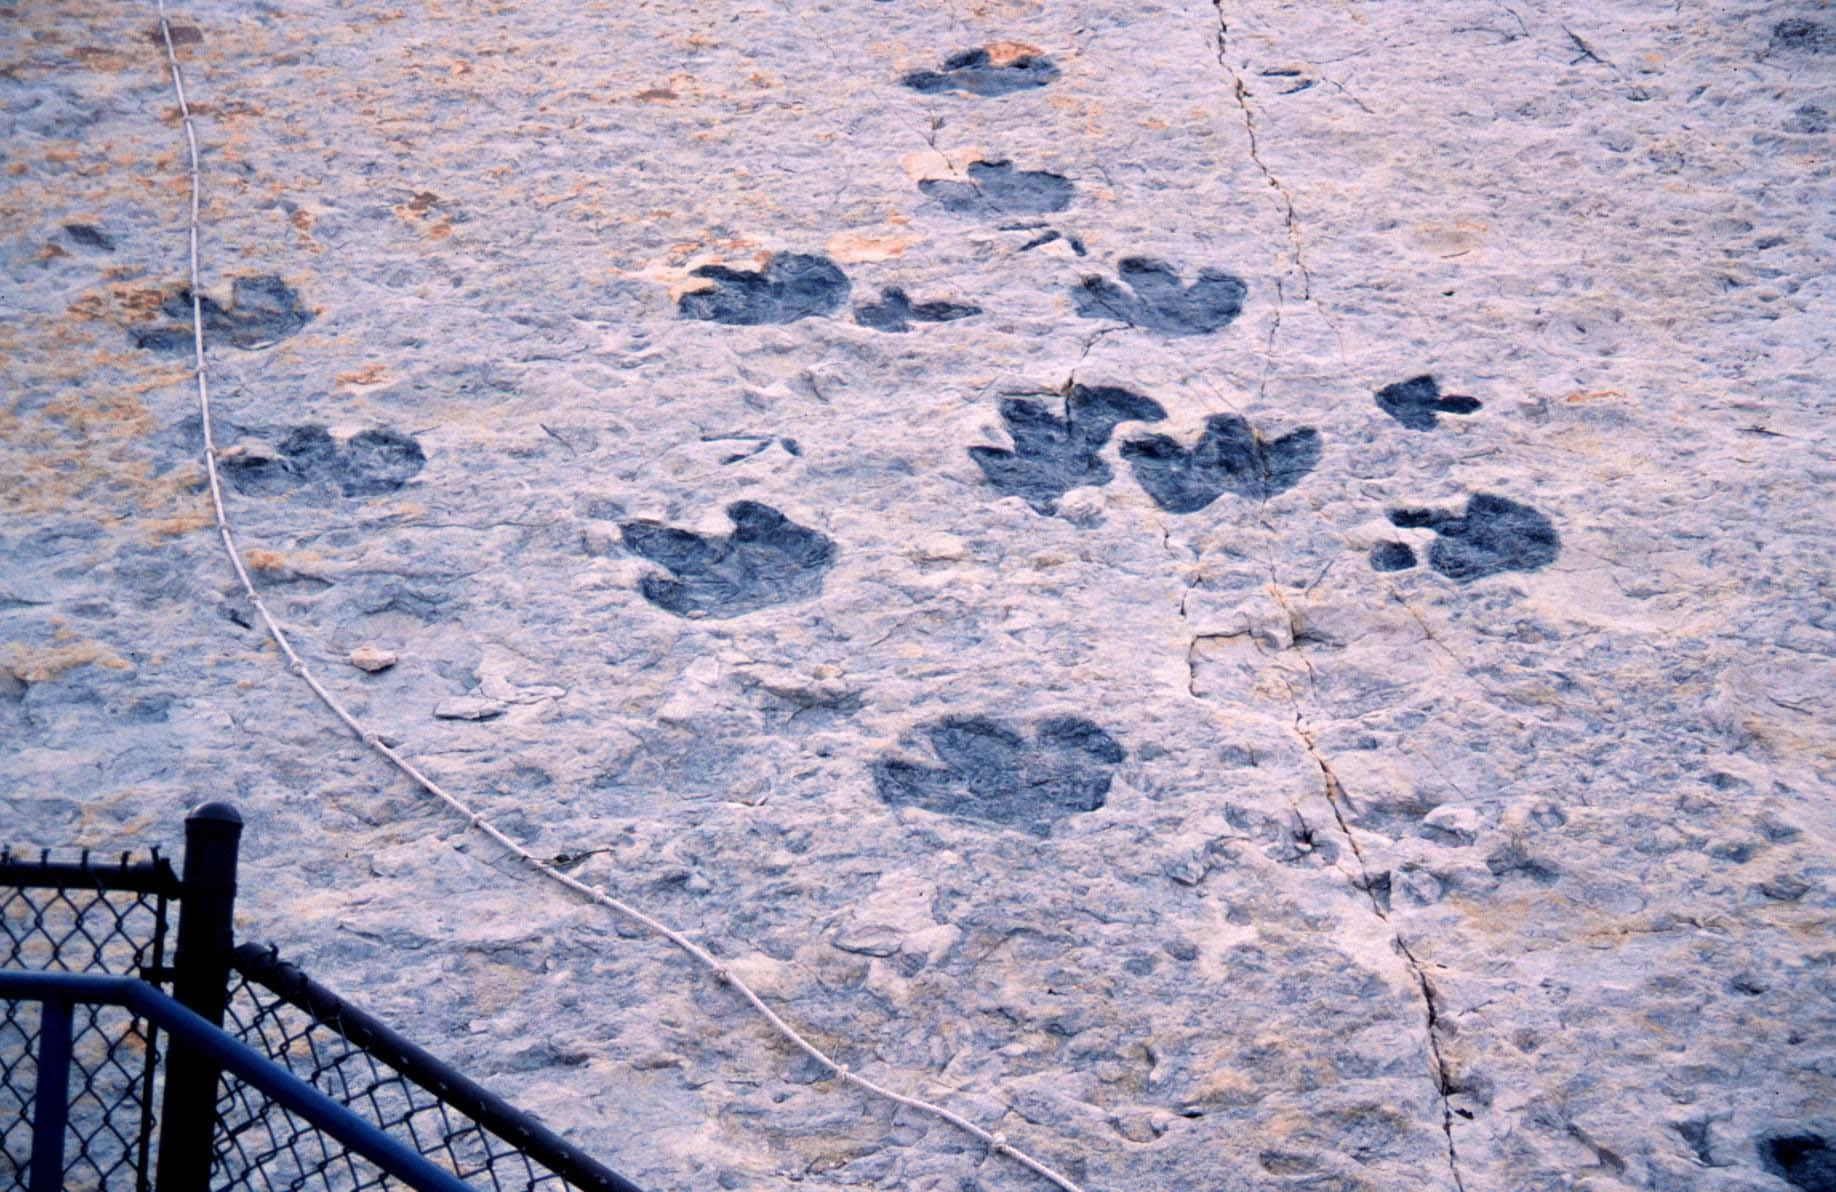
\includegraphics[width=0.62\linewidth]{images/book1/g7-dinosaur-tracks.jpg}

{\small Des empreintes de dinosaures à Dinosaur Ridge, près de Morrison,
dans le Colorado (États-Unis)~: des dizaines de pistes laissées dans un
sol mou, devenu aujourd'hui une surface de \omterm{def:g3:stones-pebbles-sand:rock}{roche} inclinée. La plupart ont
été laissées par des dinosaures herbivores, quelques-unes par des
carnivores aux doigts fins. Photographie~: Dexter Perkins (CC0, via
Wikimedia Commons).}
% ledger: commons:dino-tracks
\label{fig:g7:sediments-and-fossils:tracks}
\end{omfigure}

La biologie se sert des \omterm{def:g7:sediments-and-fossils:fossil}{fossiles} pour suivre la longue histoire des êtres
vivants. Dans ce livre, les \omterm{def:g7:sediments-and-fossils:fossil}{fossiles} sont des indices d'une autre
sorte~: ils nous disent à quoi ressemblait le lieu quand l'animal y
vivait.

\section{Couches et fossiles, une mémoire du passé}

Chaque couche garde les marques du lieu où elle s'est déposée. Les récifs
de corail poussent aujourd'hui dans des \omterm{def:g2:water-on-earth:ocean}{mers} chaudes, claires et peu
profondes~; les rides de courant se forment sur le \omterm{def:g3:stones-pebbles-sand:sand}{sable} en eau peu
profonde, au bord d'un \omterm{def:g1:landscapes-around-us:water}{lac}, d'une \omterm{def:g1:landscapes-around-us:water}{rivière} ou d'une \omterm{def:g2:water-on-earth:ocean}{mer}~; le charbon s'est
formé à partir des plantes d'anciennes forêts et de marais~; les
brachiopodes, les crinoïdes et les trilobites ne vivaient que dans la \omterm{def:g2:water-on-earth:ocean}{mer}.
Quand on retrouve les mêmes indices dans une couche ancienne, le lieu
ressemblait probablement à cela quand la couche s'est formée.
% ledger: noaa:coral-where, nps:ripple-marks, nps:ripples-shallow, usgs:coal-origin, nps:trilobite

\begin{center}
\small
\begin{tabular}{|p{0.36\linewidth}|p{0.52\linewidth}|}
\hline
\textbf{indice dans la couche} & \textbf{le lieu quand la couche s'est formée} \\
\hline
coraux & une \omterm{def:g2:water-on-earth:ocean}{mer} chaude, peu profonde et claire \\
\hline
coquilles d'animaux marins (brachiopodes, crinoïdes, trilobites) & une \omterm{def:g2:water-on-earth:ocean}{mer} \\
\hline
rides de courant à la surface d'une couche & eau peu profonde, au bord d'un \omterm{def:g1:landscapes-around-us:water}{lac}, d'une \omterm{def:g1:landscapes-around-us:water}{rivière} ou d'une \omterm{def:g2:water-on-earth:ocean}{mer} \\
\hline
empreintes de pas & \omterm{def:g3:stones-pebbles-sand:sand}{boue} ou \omterm{def:g3:stones-pebbles-sand:sand}{sable} mous et humides, souvent sur un rivage ou une berge \\
\hline
charbon & une forêt marécageuse ou un marais \\
\hline
feuilles et ailes de libellule & la terre ferme, couverte de plantes \\
\hline
\end{tabular}
\end{center}
% ledger: noaa:coral-where, nps:grca-fossils, nps:trilobite, nps:ripple-marks, nps:ripples-shallow, ucmp:footprints, usgs:coal-origin

\begin{method}[Lire une couche]\label{met:g7:sediments-and-fossils:reading}
\begin{enumerate}
  \item Regarde les grains~: les grains grossiers se déposent là où l'eau
        va vite, la \omterm{def:g3:stones-pebbles-sand:sand}{boue} fine seulement là où elle est calme.
  \item Cherche les \omterm{def:g7:sediments-and-fossils:fossil}{fossiles} et les marques (coraux, coquilles, empreintes,
        rides de courant, débris de plantes, charbon) et utilise le tableau
        ci-dessus.
  \item Rassemble les indices en une seule image du lieu~: terre ou \omterm{def:g2:water-on-earth:ocean}{mer},
        eau peu profonde ou profonde, calme ou agitée.
\end{enumerate}
\end{method}

\begin{omfigure}
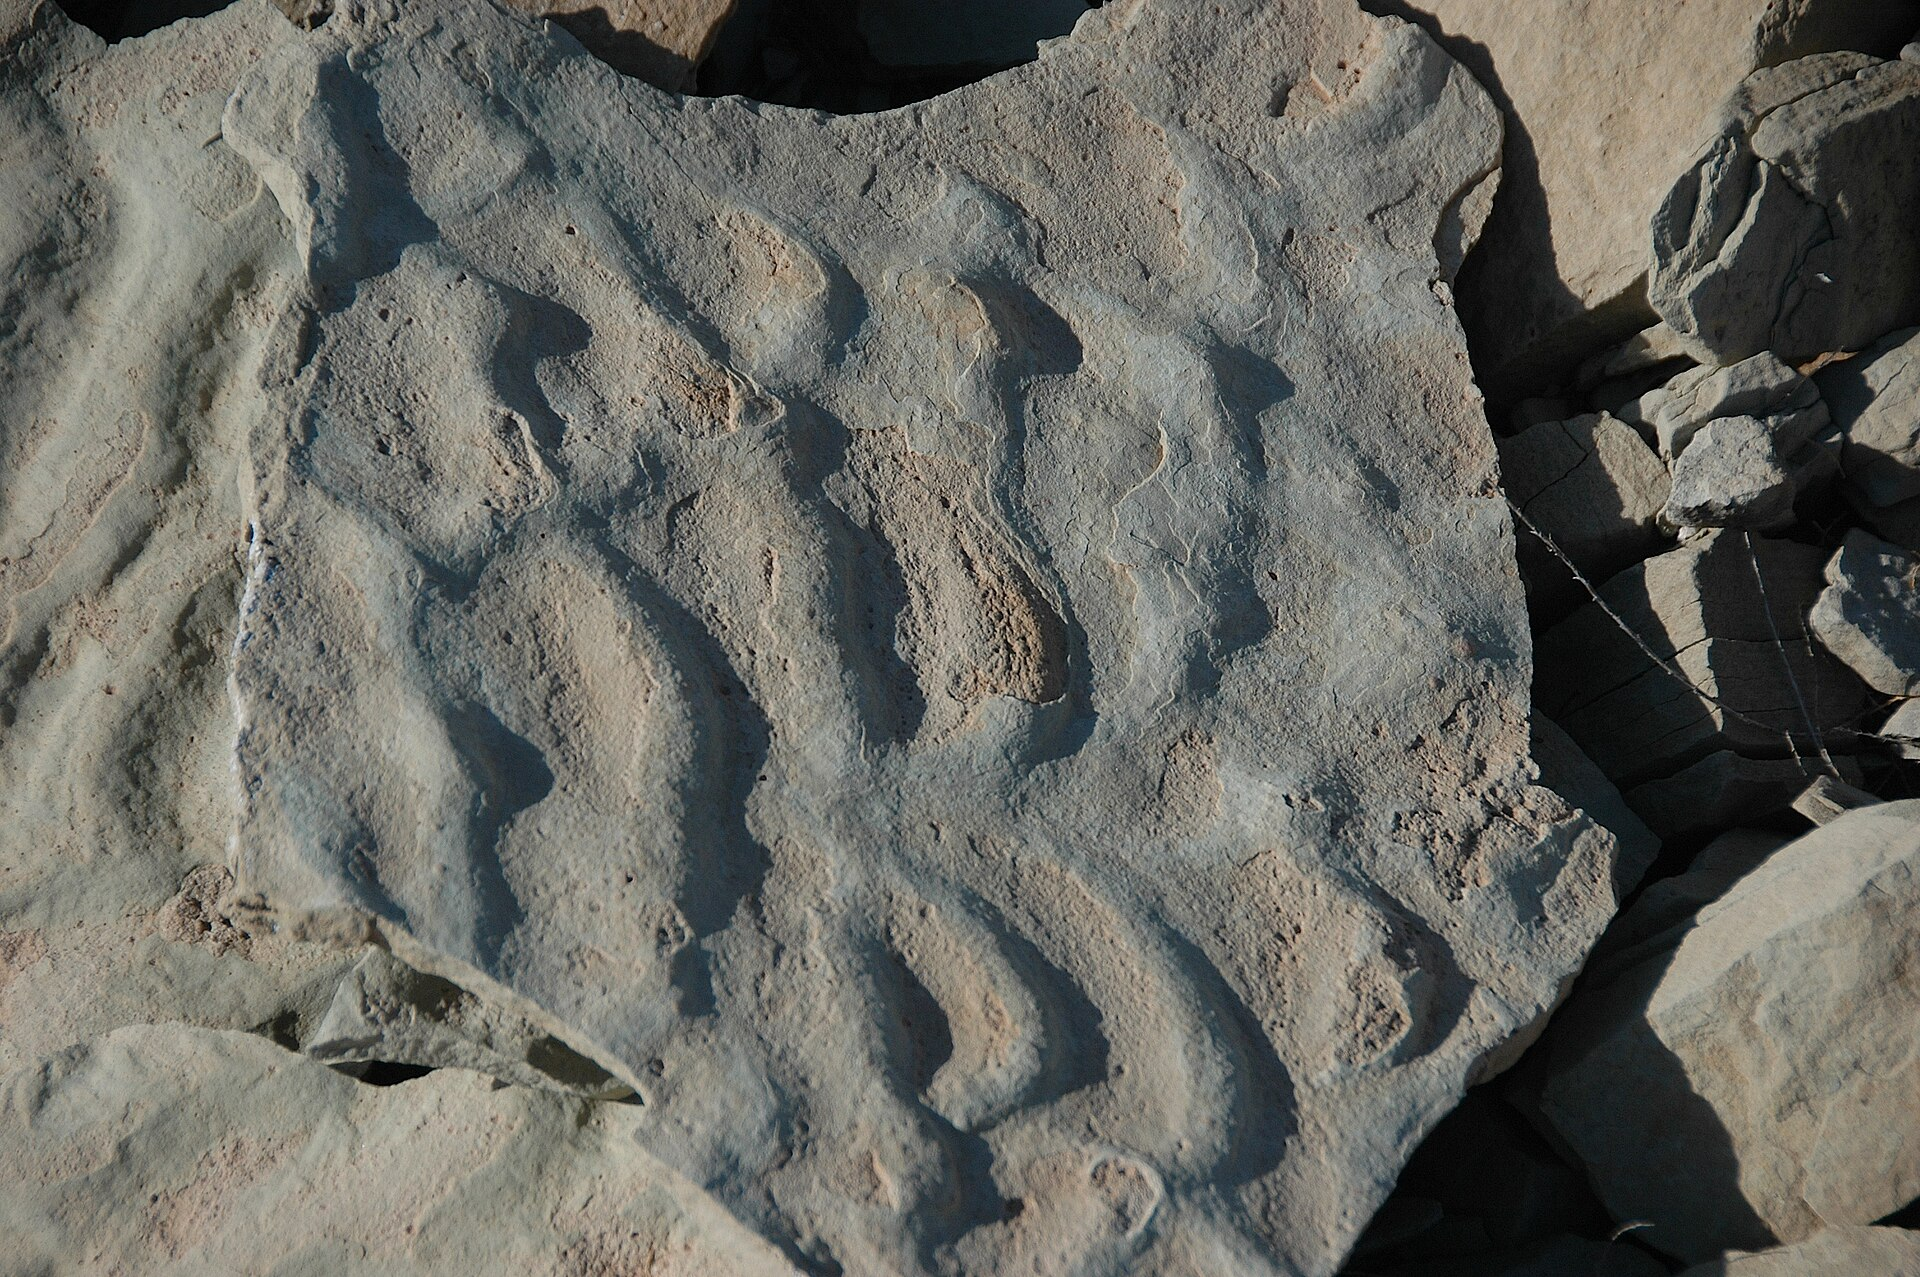
\includegraphics[width=0.56\linewidth]{images/book1/g7-ripple-marks.jpg}

{\small Des rides de courant sur une dalle de grès, dans le parc national
de Capitol Reef, en Utah (États-Unis)~: le \omterm{def:g3:stones-pebbles-sand:sand}{sable} a jadis été ridé par de
l'eau en mouvement, comme le \omterm{def:g3:stones-pebbles-sand:sand}{sable} d'une plage ou le lit d'un ruisseau
aujourd'hui. Photographie~: James St.~John (CC BY 2.0, via Wikimedia
Commons).}
% ledger: commons:ripples, nps:ripple-marks
\label{fig:g7:sediments-and-fossils:ripples}
\end{omfigure}

\begin{example}[Le sommet du Grand Canyon]\label{ex:g7:sediments-and-fossils:kaibab}
Le calcaire de Kaibab, la couche du sommet du Grand Canyon, est plein de
coquilles de brachiopodes et de morceaux de tiges de crinoïdes, deux
animaux marins. Il s'est formé sur le fond d'une \omterm{def:g2:water-on-earth:ocean}{mer}. Aujourd'hui, cette
même couche se trouve jusqu'à environ \qty{2700}{m} (\num{9000}~pieds)
au-dessus du \omterm{def:g4:world-physical-map:altitude}{niveau de la mer}~: depuis sa formation, toute la région a été
soulevée.
% ledger: nps:grca-fossils, nps:grca-kaibab
\end{example}

On peut dessiner une pile de couches sous la forme d'une \emph{colonne}~:
les couches empilées dans l'ordre où elles se sont formées, avec leur
épaisseur à l'échelle et leurs indices notés à côté. La colonne des
collines de Varden, la région inventée des exercices de cette collection,
est donnée ci-dessous.

\begin{omfigure}
\begin{tikzpicture}
  \begin{axis}[width=4.2cm, height=9.2cm, scale only axis=false, xmin=0, xmax=1, ymin=-60, ymax=485,
      axis x line=none, axis y line*=left, ytick={0,100,200,300,400},
      ylabel={mètres au-dessus de la base du grès}, label style={font=\footnotesize},
      tick label style={font=\scriptsize}, clip=false]
    \addplot[lith schist, draw=black!70, line width=0.3pt] table {figdata/out/grade-7-varden_column-unit-older.dat};
    \addplot[lith sandstone, draw=black!70, line width=0.3pt] table {figdata/out/grade-7-varden_column-unit-sandstone.dat};
    \addplot[lith limestone, draw=black!70, line width=0.3pt] table {figdata/out/grade-7-varden_column-unit-limestone.dat};
    \addplot[lith shale, draw=black!70, line width=0.3pt] table {figdata/out/grade-7-varden_column-unit-shale.dat};
    \addplot[om lith={white}{om limestone}, draw=black!70, line width=0.3pt] table {figdata/out/grade-7-varden_column-unit-chalk.dat};
    \node[anchor=west, align=left, font=\footnotesize] at (axis cs:1.12,450) {\textbf{craie}~: son sommet a été\\usé (seule sa base est dessinée)};
    \node[anchor=west, align=left, font=\footnotesize] at (axis cs:1.12,350) {\textbf{argilite}, \qty{100}{m}~: grains très fins~;\\ammonites};
    \node[anchor=west, align=left, font=\footnotesize] at (axis cs:1.12,210) {\textbf{calcaire}, \qty{180}{m}~:\\coraux et coquilles};
    \node[anchor=west, align=left, font=\footnotesize] at (axis cs:1.12,60) {\textbf{grès}, \qty{120}{m}~:\\rides de courant, empreintes};
    \node[anchor=west, align=left, font=\footnotesize] at (axis cs:1.12,-30) {roches plus anciennes (schiste et granite),\\usées à plat avant l'arrivée du grès};
  \end{axis}
\end{tikzpicture}

\medskip
{\small La colonne des collines de Varden, la région inventée de cette
collection~: les couches dans l'ordre où elles se sont formées, la
première en bas, avec leurs épaisseurs à l'échelle. Les \omterm{def:g7:sediments-and-fossils:fossil}{fossiles} et les
marques notés à côté sont des données d'exercice.}
% ledger: (invented region: figdata/shared/region.py, drawn by figdata/grade-7/varden_column.py)
\label{fig:g7:sediments-and-fossils:column}
\end{omfigure}

\begin{omfigure}
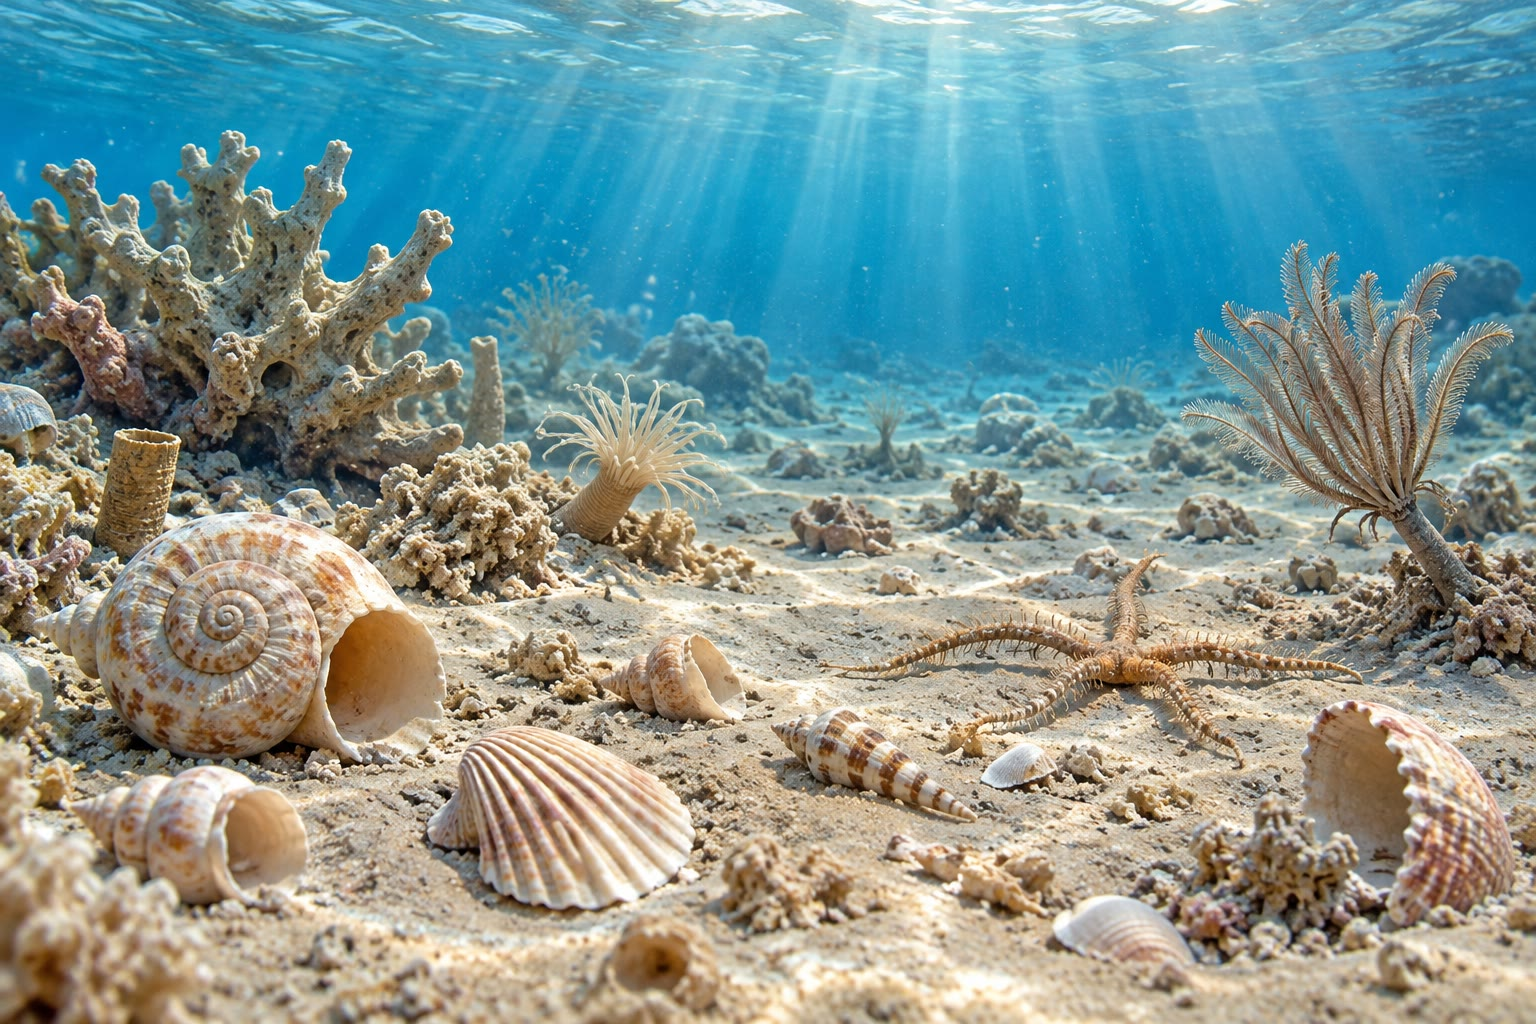
\includegraphics[width=0.6\linewidth]{images/book1/ai/g7-shallow-sea.jpg}

{\small Un fond de \omterm{def:g2:water-on-earth:ocean}{mer} chaud et peu profond d'autrefois, tel qu'il pouvait
être pendant que des coquilles et des morceaux de corail se déposaient
pour former un futur calcaire (illustration générée par IA d'une scène
générique).}
\label{fig:g7:sediments-and-fossils:shallow-sea}
\end{omfigure}

\begin{remark}[Regarder, photographier, laisser en place]\label{rem:g7:sediments-and-fossils:leave}
Dans de nombreux lieux protégés, il est interdit d'emporter un \omterm{def:g7:sediments-and-fossils:fossil}{fossile}~:
dans le Grand Canyon, par exemple, la loi interdit de déterrer, de déplacer
ou d'emporter le moindre \omterm{def:g7:sediments-and-fossils:fossil}{fossile}. Un visiteur qui en trouve un le
photographie ou le dessine, le laisse en place pour que d'autres le voient
et que les scientifiques l'étudient, et prévient un garde du parc.
\end{remark}
% ledger: nps:grca-fossils

\begin{inthefield}[Des sédiments qui se déposent aujourd'hui]
Sur une plage, au bord d'un \omterm{def:g1:landscapes-around-us:water}{lac} ou sur la berge d'un ruisseau, avec un
adulte, regarde le \omterm{def:g3:stones-pebbles-sand:sand}{sable} sous une eau peu profonde~: l'eau en mouvement le
façonne en rides, comme celles que garde le vieux grès. Laisse une
empreinte de pas dans le \omterm{def:g3:stones-pebbles-sand:sand}{sable} mouillé, près du bord de l'eau, et regarde
ce qu'en font les vagues suivantes. Après une journée de \omterm{def:g4:clouds-rain-snow:precipitation}{pluie}, regarde
une flaque qui a séché~: une fine pellicule de \omterm{def:g3:stones-pebbles-sand:sand}{boue} recouvre souvent le
\omterm{def:g3:stones-pebbles-sand:sand}{sable} du fond --- les grains les plus fins se sont déposés en dernier,
quand l'eau était immobile. Dessine ce que tu vois, et note où et quand.
\end{inthefield}
% ledger: nps:ripple-marks, ucmp:footprints, usgs:strata

\section{Exercices}

\begin{exercise}[$\star$]\label{exo:g7:sediments-and-fossils:1}
Associe chaque mot à sa définition~: \omterm{def:g7:sediments-and-fossils:sediment}{sédiment}~; \omterm{def:g7:sediments-and-fossils:layer}{strate}~; \omterm{def:g7:sediments-and-fossils:fossil}{fossile}~;
\omterm{def:g7:sediments-and-fossils:fossil}{moule}~; \omterm{def:g7:sediments-and-fossils:fossil}{moulage}~; \omterm{def:g7:sediments-and-fossils:fossil}{trace fossile}. (a) Un creux laissé dans une \omterm{def:g3:stones-pebbles-sand:rock}{roche} là où
une coquille s'est dissoute. (b) Une empreinte de pas ou un terrier
conservés dans une \omterm{def:g3:stones-pebbles-sand:rock}{roche}. (c) Un matériau meuble déposé par l'eau, le vent
ou la glace. (d) Une copie en pierre formée quand un creux se remplit de
\omterm{def:g6:rocks-and-minerals:mineral}{minéraux}. (e) Une nappe de \omterm{def:g7:sediments-and-fossils:sediment}{sédiment} déposée en une seule fois. (f) Le
reste ou la trace d'un être vivant d'autrefois, conservé dans la \omterm{def:g3:stones-pebbles-sand:rock}{roche}.
\end{exercise}

\begin{exercise}[$\star$]\label{exo:g7:sediments-and-fossils:2}
Remets ces étapes dans l'ordre, pour raconter comment une coquille devient
un \omterm{def:g7:sediments-and-fossils:fossil}{fossile} à la surface~: (a) l'\omterm{def:g5:water-shapes-the-land:erosion}{érosion} use les couches qui la
recouvrent~; (b) l'animal meurt sur le fond de la \omterm{def:g2:water-on-earth:ocean}{mer}~; (c) de nouvelles
couches s'entassent et la coquille se change en pierre~; (d) la \omterm{def:g3:stones-pebbles-sand:sand}{boue}
recouvre vite la coquille.
\end{exercise}

\begin{exercise}[$\star$]\label{exo:g7:sediments-and-fossils:3}
Utilise le tableau des indices. Où chaque couche s'est-elle formée~? (a)
Un calcaire plein de coraux. (b) Un grès dont la surface montre des rides
de courant. (c) Une couche sombre de charbon. (d) Une argilite avec des
empreintes de feuilles et une aile de libellule.
\end{exercise}

\begin{exercise}[$\star$]\label{exo:g7:sediments-and-fossils:4}
Vrai ou faux~? Corrige les phrases fausses. (a) Tout animal qui meurt
devient un jour un \omterm{def:g7:sediments-and-fossils:fossil}{fossile}. (b) Une empreinte de pas peut être un \omterm{def:g7:sediments-and-fossils:fossil}{fossile}.
(c) Quand une eau boueuse ralentit, la \omterm{def:g3:stones-pebbles-sand:sand}{boue} fine se dépose en premier. (d)
Les \omterm{def:g7:sediments-and-fossils:sediment}{sédiments} se déposent à plat.
\end{exercise}

\begin{exercise}[$\star\star$]\label{exo:g7:sediments-and-fossils:5}
Utilise la colonne des collines de Varden. (a) Donne l'épaisseur du grès,
du calcaire et de l'argilite. (b) Quelle est leur épaisseur totale~? (c)
Quel pourcentage de ce total représente le calcaire~? Arrondis à l'unité.
(d) Pourquoi la colonne ne donne-t-elle aucune épaisseur pour la craie~?
\end{exercise}

\begin{exercise}[$\star\star$]\label{exo:g7:sediments-and-fossils:6}
Une élève secoue un bocal d'eau avec du gravier, du \omterm{def:g3:stones-pebbles-sand:sand}{sable} et de la \omterm{def:g3:stones-pebbles-sand:sand}{boue},
puis laisse reposer. (a) Dessine le bocal le lendemain, et légende les
couches. (b) Pourquoi l'eau est-elle encore trouble au bout d'une
heure~? (c) Elle ajoute encore du \omterm{def:g3:stones-pebbles-sand:sand}{sable} et de la \omterm{def:g3:stones-pebbles-sand:sand}{boue} et laisse reposer.
Que voit-elle maintenant au fond~? (d) Quelle couche du bocal s'est formée
en premier~?
\end{exercise}

\begin{exercise}[$\star\star$]\label{exo:g7:sediments-and-fossils:7}
Lequel de ces restes a le plus de chances de devenir un \omterm{def:g7:sediments-and-fossils:fossil}{fossile}, et lequel
en a le moins~? Explique. (a) Une méduse rejetée sur un rivage rocheux.
(b) Une coquille d'escargot enfouie dans la \omterm{def:g3:stones-pebbles-sand:sand}{boue} d'un \omterm{def:g1:landscapes-around-us:water}{lac} calme. (c) Un os
resté des années sur une \omterm{def:g1:landscapes-around-us:landform}{plaine} sèche. (d) Une coquille de palourde
recouverte de \omterm{def:g3:stones-pebbles-sand:sand}{sable} lors d'une \omterm{def:g5:water-shapes-the-land:flood}{crue}.
\end{exercise}

\begin{exercise}[$\star\star$]\label{exo:g7:sediments-and-fossils:8}
Une coquille est enfouie dans du \omterm{def:g3:stones-pebbles-sand:sand}{sable} qui devient du grès. L'eau qui
s'infiltre dans la \omterm{def:g3:stones-pebbles-sand:rock}{roche} dissout complètement la coquille. (a) Que
reste-t-il dans la \omterm{def:g3:stones-pebbles-sand:rock}{roche}~? (b) Plus tard, des \omterm{def:g6:rocks-and-minerals:mineral}{minéraux} remplissent ce
creux. Que se forme-t-il~? (c) La coquille elle-même est-elle encore
là~? (d) Pourquoi trouve-t-on plus souvent des \omterm{def:g7:sediments-and-fossils:fossil}{moules} et des \omterm{def:g7:sediments-and-fossils:fossil}{moulages}
dans le grès que dans l'argilite~? (Pense à la facilité avec laquelle
l'eau passe entre les grains.)
\end{exercise}

\begin{exercise}[$\star\star$]\label{exo:g7:sediments-and-fossils:9}
Le Grand Canyon a une profondeur moyenne de \qty{1.6}{km}. (a) Écris
cette profondeur en mètres. (b) Suppose que les parois du canyon soient
faites de couches de \qty{80}{m} d'épaisseur chacune~: combien de couches
tiendraient entre le bord et le fond~? (c) Quel pourcentage de la
profondeur représente une couche de \qty{160}{m}~?
\end{exercise}

\begin{exercise}[$\star\star$]\label{exo:g7:sediments-and-fossils:10}
On trouve des empreintes de dinosaures dans un grès. (a) Les dinosaures
marchaient-ils sur de la \omterm{def:g3:stones-pebbles-sand:rock}{roche} dure~? Explique. (b) Pourquoi la plupart des
empreintes laissées sur un rivage boueux disparaissent-elles~? (c) Que
fallait-il qu'il se passe peu après le passage des dinosaures pour que les
empreintes soient conservées~? (d) Une empreinte est-elle un \omterm{def:g7:sediments-and-fossils:fossil}{fossile} du
corps ou une \omterm{def:g7:sediments-and-fossils:fossil}{trace fossile}~?
\end{exercise}

\begin{exercise}[$\star\star\star$]\label{exo:g7:sediments-and-fossils:11}
Dans un \omterm{def:g1:landscapes-around-us:water}{lac}, chaque \omterm{def:g5:water-shapes-the-land:flood}{crue} laisse une couche de \omterm{def:g3:stones-pebbles-sand:sand}{sable} d'environ \qty{2}{cm}
d'épaisseur, et les semaines calmes qui suivent une couche de \omterm{def:g3:stones-pebbles-sand:sand}{boue}
d'environ \qty{5}{mm} d'épaisseur (données d'exercice). (a) Quelle est
l'épaisseur, en millimètres, d'une paire de couches~? (b) Une carotte
prélevée au fond du \omterm{def:g1:landscapes-around-us:water}{lac} mesure \qty{1}{m} de long et n'est faite que de
telles paires. Combien de \omterm{def:g5:water-shapes-the-land:flood}{crues} enregistre-t-elle~? (c) Près de
l'\omterm{def:g5:water-shapes-the-land:source-mouth}{embouchure} de la \omterm{def:g1:landscapes-around-us:water}{rivière}, les couches de \omterm{def:g3:stones-pebbles-sand:sand}{sable} sont plus épaisses~; au
large, elles sont plus fines. Explique pourquoi. (d) Pourquoi y a-t-il plus
de \omterm{def:g3:stones-pebbles-sand:sand}{boue} que de \omterm{def:g3:stones-pebbles-sand:sand}{sable} loin de l'\omterm{def:g5:water-shapes-the-land:source-mouth}{embouchure}~?
\end{exercise}

\begin{exercise}[$\star\star\star$]\label{exo:g7:sediments-and-fossils:12}
Les \omterm{def:g7:sediments-and-fossils:fossil}{fossiles} trouvés dans les \omterm{def:g3:stones-pebbles-sand:rock}{roches} sont surtout des coquilles et de
minuscules restes~; les \omterm{def:g7:sediments-and-fossils:fossil}{fossiles} d'animaux mous sont rares, et les
dinosaures ne sont qu'une toute petite partie de tous les \omterm{def:g7:sediments-and-fossils:fossil}{fossiles}. (a)
Explique pourquoi les coquilles sont si fréquentes. (b) Explique pourquoi
les animaux mous sont rares. (c) Une scientifique veut connaître tous les
animaux qui vivaient dans une \omterm{def:g2:water-on-earth:ocean}{mer} ancienne. Les \omterm{def:g7:sediments-and-fossils:fossil}{fossiles} peuvent-ils lui
en donner la liste complète~? Explique.
\end{exercise}

\section{Problème~: La colonne des collines de Varden}

\begin{problem}[{Problème du week-end --- les couches des collines de Varden sont
lues une à une, leurs fossiles disent où elles se sont formées, et l'on
calcule le temps qu'il a fallu pour empiler le calcaire}]
\label{pb:g7:sediments-and-fossils:1}
% ledger: (invented region: figdata/shared/region.py; rates are exercise data, figdata/grade-7/varden_column.py part rates)
Utilise la colonne des collines de Varden de ce chapitre. Son grès montre
des rides de courant et des empreintes~; son calcaire contient des coraux
et des coquilles~; son argilite est faite de grains très fins, avec des
ammonites~; la craie du sommet a été en partie usée.

\medskip
\noindent\textbf{Partie I --- Lire les couches.}\par\nopagebreak
\begin{enumerate}[beginpenalty=10000]
  \item Donne la liste des quatre couches, de la première déposée à la
        dernière.
  \item Donne l'épaisseur du grès, du calcaire et de l'argilite, et leur
        total.
  \item Quel pourcentage de ce total représente le calcaire~?
  \item Pourquoi personne ne peut-il dire quelle était l'épaisseur de la
        craie quand elle s'est formée~?
\end{enumerate}

\medskip
\noindent\textbf{Partie II --- Les fossiles qu'elles contiennent.}\par\nopagebreak
\begin{enumerate}[resume, beginpenalty=10000]
  \item Où le grès s'est-il formé~? Donne deux indices.
  \item Où le calcaire s'est-il formé~? Donne l'indice.
  \item L'argilite est faite de grains très fins. L'eau était-elle calme ou
        agitée quand elle s'est déposée~? Explique.
  \item Raconte l'histoire du lieu en trois phrases, du grès à l'argilite.
\end{enumerate}

\medskip
\noindent\textbf{Partie III --- Le temps qu'il a fallu.}\par\nopagebreak
\begin{enumerate}[resume, beginpenalty=10000]
  \item Écris l'épaisseur du calcaire en centimètres.
  \item Suppose que le grès se soit empilé de \qty{1}{cm} tous les 20~ans.
        Combien d'années ses \qty{120}{m} ont-ils demandé~?
  \item Suppose que le calcaire se soit empilé de \qty{1}{cm} tous les
        100~ans. Combien d'années \qty{1}{m} de calcaire a-t-il demandé~?
  \item Combien d'années les \qty{180}{m} de calcaire ont-ils demandé~?
        Combien de fois plus longtemps que pour le grès~?
\end{enumerate}
\end{problem}
